\chapter{Introduction}

Industrial robots have become an inseparable part of the manufacturing process in large enterprises. In small to medium-sized enterprises (SMEs), the adoption of robots has been slower, mainly due to high entry costs and difficult reprogramming. Having the ability to quickly and easily reprogram industrial robots would accelerate their adoption in SMEs, and allow them to be used in more flexible scenarios. The ARCOR2 system~\cite{kapinus2023arcor2}, along with the Android application, AREditor, aims to streamline the reprogramming process by utilizing augmented reality and a tablet device.  However, the options for setting a pose of the robot in the app are limited and hinder its usability. 

When programming robots in AREditor, the user uses the robot arm to define points in space. When working with collaborative robots, the operator can reposition the robot manually -- by grabbing the robot arm and dragging it to the desired spot. This task becomes more tedious when the robot cannot be moved by hand. AREditor provides incremental stepping functionality, allowing the user to move the robot arm by selected increment in the direction of a chosen axis. This is sufficient for minor tweaking and fine-tuning, but becomes too slow when a more substantial repositioning is necessary. Another problem is the lack of visualization of the final pose. 

This thesis proposes a novel system for the rapid positioning of a robot, employing a model robot rendered on-screen over the real robot in the workspace. Through this approach, the user can directly manipulate the model without affecting the robot, which allows for a safe interaction, unconstrained by the movement speed limit of the particular robot. Another benefit of this approach is the ability to visualize different poses before committing to a final one, thus saving time repositioning. 

The thesis is structured as follows: In the first chapter, a brief summary of related research is presented. The second chapter contains a rundown of the ARCOR2 system and the related user interface AREditor. In the following chapters, the design and implementation of the final system is described. Finally, the results of the user testing are presented and evaluated. 

\chapter{Related Work}
With rising interest in industrial robots, the simplification of robot programming has been at the forefront for many researchers. Suzuki et al.~\cite{suzuki2022augmented} compiled 460 papers on AR-enabled human-robot interaction (AR-HRI), categorizing the works into various categories. The survey has shown that most of the research is focused on facilitating programming and supporting real-time control. When it comes to devices, however, most researchers favor on-body, wearable devices (especially head-mounted displays) over handhelds. 

\section{Wearable devices}
Head-mounted displays (HMDs) provide an immersive experience and free up the operator's hands, allowing them to perform work while always having crucial information in their field of vision. However, the lack of a tangible device in the hands of the user raises the question of how they will interact with the workplace. Popular approaches include gestures \cite{voicelargescale, handsfree, packing}, handheld pointers \cite{2009, speared}, and less commonly voice commands \cite{voicelargescale}. Park et al.~\cite{handsfree} propose a hands-free system utilizing head gestures and gaze for selection and interaction. Chan et al.~\cite{voicelargescale} created an interface allowing the user to set trajectory points on the work surface using a combination of gaze and voice commands. Ong et al.~\cite{ONG2020101820} combine a stereoscopic HMD with a physical handheld pointer, representing the end effector. In this instance, the display is created by combining a VR headset and two webcams mounted directly onto it. A much more prevalent approach is to use a see-through AR headset, such as the Microsoft HoloLens. The SPEARED framework by Yigitbas et al.\cite{speared} uses HoloLens to display the current robot working state and detected objects, but also the current program in the form of code blocks, which can be modified in the AR environment. In the case of SPEARED, there is no direct robot pose manipulation, all interaction is conducted through code. Chan et al.\cite{voicelargescale} also utilize Microsoft HoloLens, but allow the user to directly set trajectories by using a combination of gaze and voice commands. 


\section{Handheld devices}

While there have been works focusing on AR-enabled robot programming systems for handheld devices, they certainly represent a minority, especially concerning direct robot pose manipulation. The interface often only allows the user to program 'pick and place' tasks, or the robot is programmed kinesthetically\cite{picknplace, Tango}.

Pertaining to controlling the robot pose explicitly, two main approaches can be discerned: individual joint setting and end effector location setting. Setting each joint rotation individually is not suitable for end users lacking experience with robotics, and even skilled operators rarely utilize it. Most implementations, however, provide both options. An earlier work by Frank et al.\cite{planar} developed a system to control a planar robot on a tablet device, which provides the user with the ability to control both end effector location and individual angles through tapping and dragging on the screen. Zhang et al.~\cite{ZHANG20201221} provide the user with a set of arrows to control each joint separately, or to command the end effector directly, with a similar approach being taken in some older works~\cite{pendant}. 



\chapter{ARCOR2}
ARCOR2 (Augmented Reality Collaborative Robot) is a framework for visual programming of industrial robots developed by the research group Robo@FIT\footnote{\url{https://www.fit.vut.cz/research/group/robo/.en}}. It enables end-users to create programs by defining points in space and program steps that are spatially visualized, allowing for an easy understanding of work processes. The system can generate code from visually defined procedures and facilitates control of its execution. Multiple robots, machines, and services can be included in a single workspace, with multiple concurrent users to be connected. New robots and services can be integrated by implementing an \texttt{Object Type} -- a plugin into the system representing an interface between ARCOR2 and a real-world object, e.g. a type of robot~\cite{kapinus2023arcor2}.

The system is divided into the back end, comprising several independent services, and the front end (in this case, AREditor)~\cite{arcor2}. The main service handling all incoming and outgoing communication is ARServer. ARServer is in charge of propagating messages to other services, holding system state, and sending out notifications upon changes. UIs such as AREditor can interact with the system state through RPCs.

\section{API}
Communication between ARServer and AREditor takes place through WebSockets. The communication protocol is based on RPCs and events, which are defined in the form of dataclasses\footnote{\url{https://docs.python.org/3/library/dataclasses.html}} and serialized into JSON.

Dataclasses are used to create an OpenAPI\footnote{\href{https://www.openapis.org/}{https://www.openapis.org/}} representation, which is subsequently used to generate C\# classes used in AREditor. In AREditor, each RPC is represented by such class in the \texttt{IO.Swagger.Model} namespace, and contains a method to serialize self to JSON.

\subsection{RPCs}
To each RPC (Remote Procedure Call) sent by AREditor, the server elicits a response. The response contains the resulting data. If the request fails, the data field is empty, and a message informing of the error. An example of a successful request-response sequence would be: 
\begin{verbatim}
    RPC request: 
    InverseKinematics.Request(
        id=28, 
        request='InverseKinematics', 
        args=InverseKinematics.Request.Args(
            robot_id='obj_edc94797032d410289f7cd241b5c6fe8', 
            end_effector_id='default', 
            pose=Pose(...), 
            start_joints=[...], 
            avoid_collisions=True, 
            arm_id=None)) 
    
    RPC response:
        InverseKinematics.Response(
            id=28, 
            response='InverseKinematics', 
            result=True, 
            messages=None, 
            data=[...])
\end{verbatim}

Note that the result field is \texttt{True}, and there is no message. Had the request failed, the response would look as follows:

\begin{verbatim}
     RPC response:
        InverseKinematics.Response(
            id=29, 
            response='InverseKinematics', 
            result=False, 
            messages=['arcor2 (General): Failed to compute IK.'], 
            data=None)
\end{verbatim}

\subsection{Events}
The main purpose of events is to notify connected user interfaces of asynchronous events. Notifications are frequently sent after an RPC has been processed. The pattern then becomes:
\begin{enumerate}
    \item RPC request
    \item RPC processed; response sent
    \item Event broadcasted
\end{enumerate}

A typical use case can be observed in robot stepping. The user sends a request to move the end effector, the end effector is moved, and after the movement is finished, an event is sent to notify AREditor and all other connected user interfaces of the changed robot pose.

\section{AREditor}
AREditor is a mobile application used to interface with ARCOR2. AREditor aims to allow users with little or no programming experience to create programs within the workspace. Within the application, users can easily interact with the robotic workspace through augmented reality. 

After connecting to ARServer, the user is presented with the main screen, from where they can create or open scenes, projects, and packages. When a scene (project, package) is opened, the application switches to the editor.

\subsection{Architecture}

AREditor comprises several singleton classes handling the most important functionality such as communication with ARServer, holding the application state, and managing the active scene or project. They provide events, to which the individual screens and menus can dynamically subscribe.

\subsubsection{\texttt{GameManager}}

\texttt{GameManager} is the main controller of the application. It manages different screens, holds the application state, holds the connection status, and notifies users of changes. Connection to ARServer is created here, using \texttt{WebsocketManager}. 

\subsubsection{\texttt{WebsocketManager}}

The \texttt{WebsocketManager} class in AREditor is responsible for communication with ARServer. It provides methods to create connection, creates and sends RPCs, holds the websocket context, processes received data and broadcasts events, informing subscribers of changes on connection status, robot pose, action objects addition/removal, etc. 

For outgoing data, each type of RPC request is represented by a class, generated by the OpenAPI Generator CLI\footnote{\href{https://openapi-generator.tech/}{https://openapi-generator.tech/}}. The class is instantiated, the data is serialized and sent through the WebSocket. The response data are awaited and deserialized using either a corresponding class, or an anonymous type\footnote{\href{https://learn.microsoft.com/en-us/dotnet/csharp/fundamentals/types/anonymous-types}{https://learn.microsoft.com/en-us/dotnet/csharp/fundamentals/types/anonymous-types}} and based on the \texttt{@event} value, the corresponding event is dispatched. 

\subsection{Editor screen}
The editor is the AR-enabled part of the application, responsible for all 3D visualization and interaction \myworries{almost word for word, should I cite?}. Available menus are listed on the left side of the screen, organized into groups, and accessible through tabs: Favorites, Add, Utility, Home, and Robot. The right side of the screen is occupied by the selector menu by default, which provides a list of action objects in the workspace. When a different menu is selected from the list, the selector menu is hidden and replaced by the corresponding menu, as pictured in \ref{fig:EditorMenus}. 

\begin{figure}
    \centering
    
        \subfloat[Selector menu, the default.]{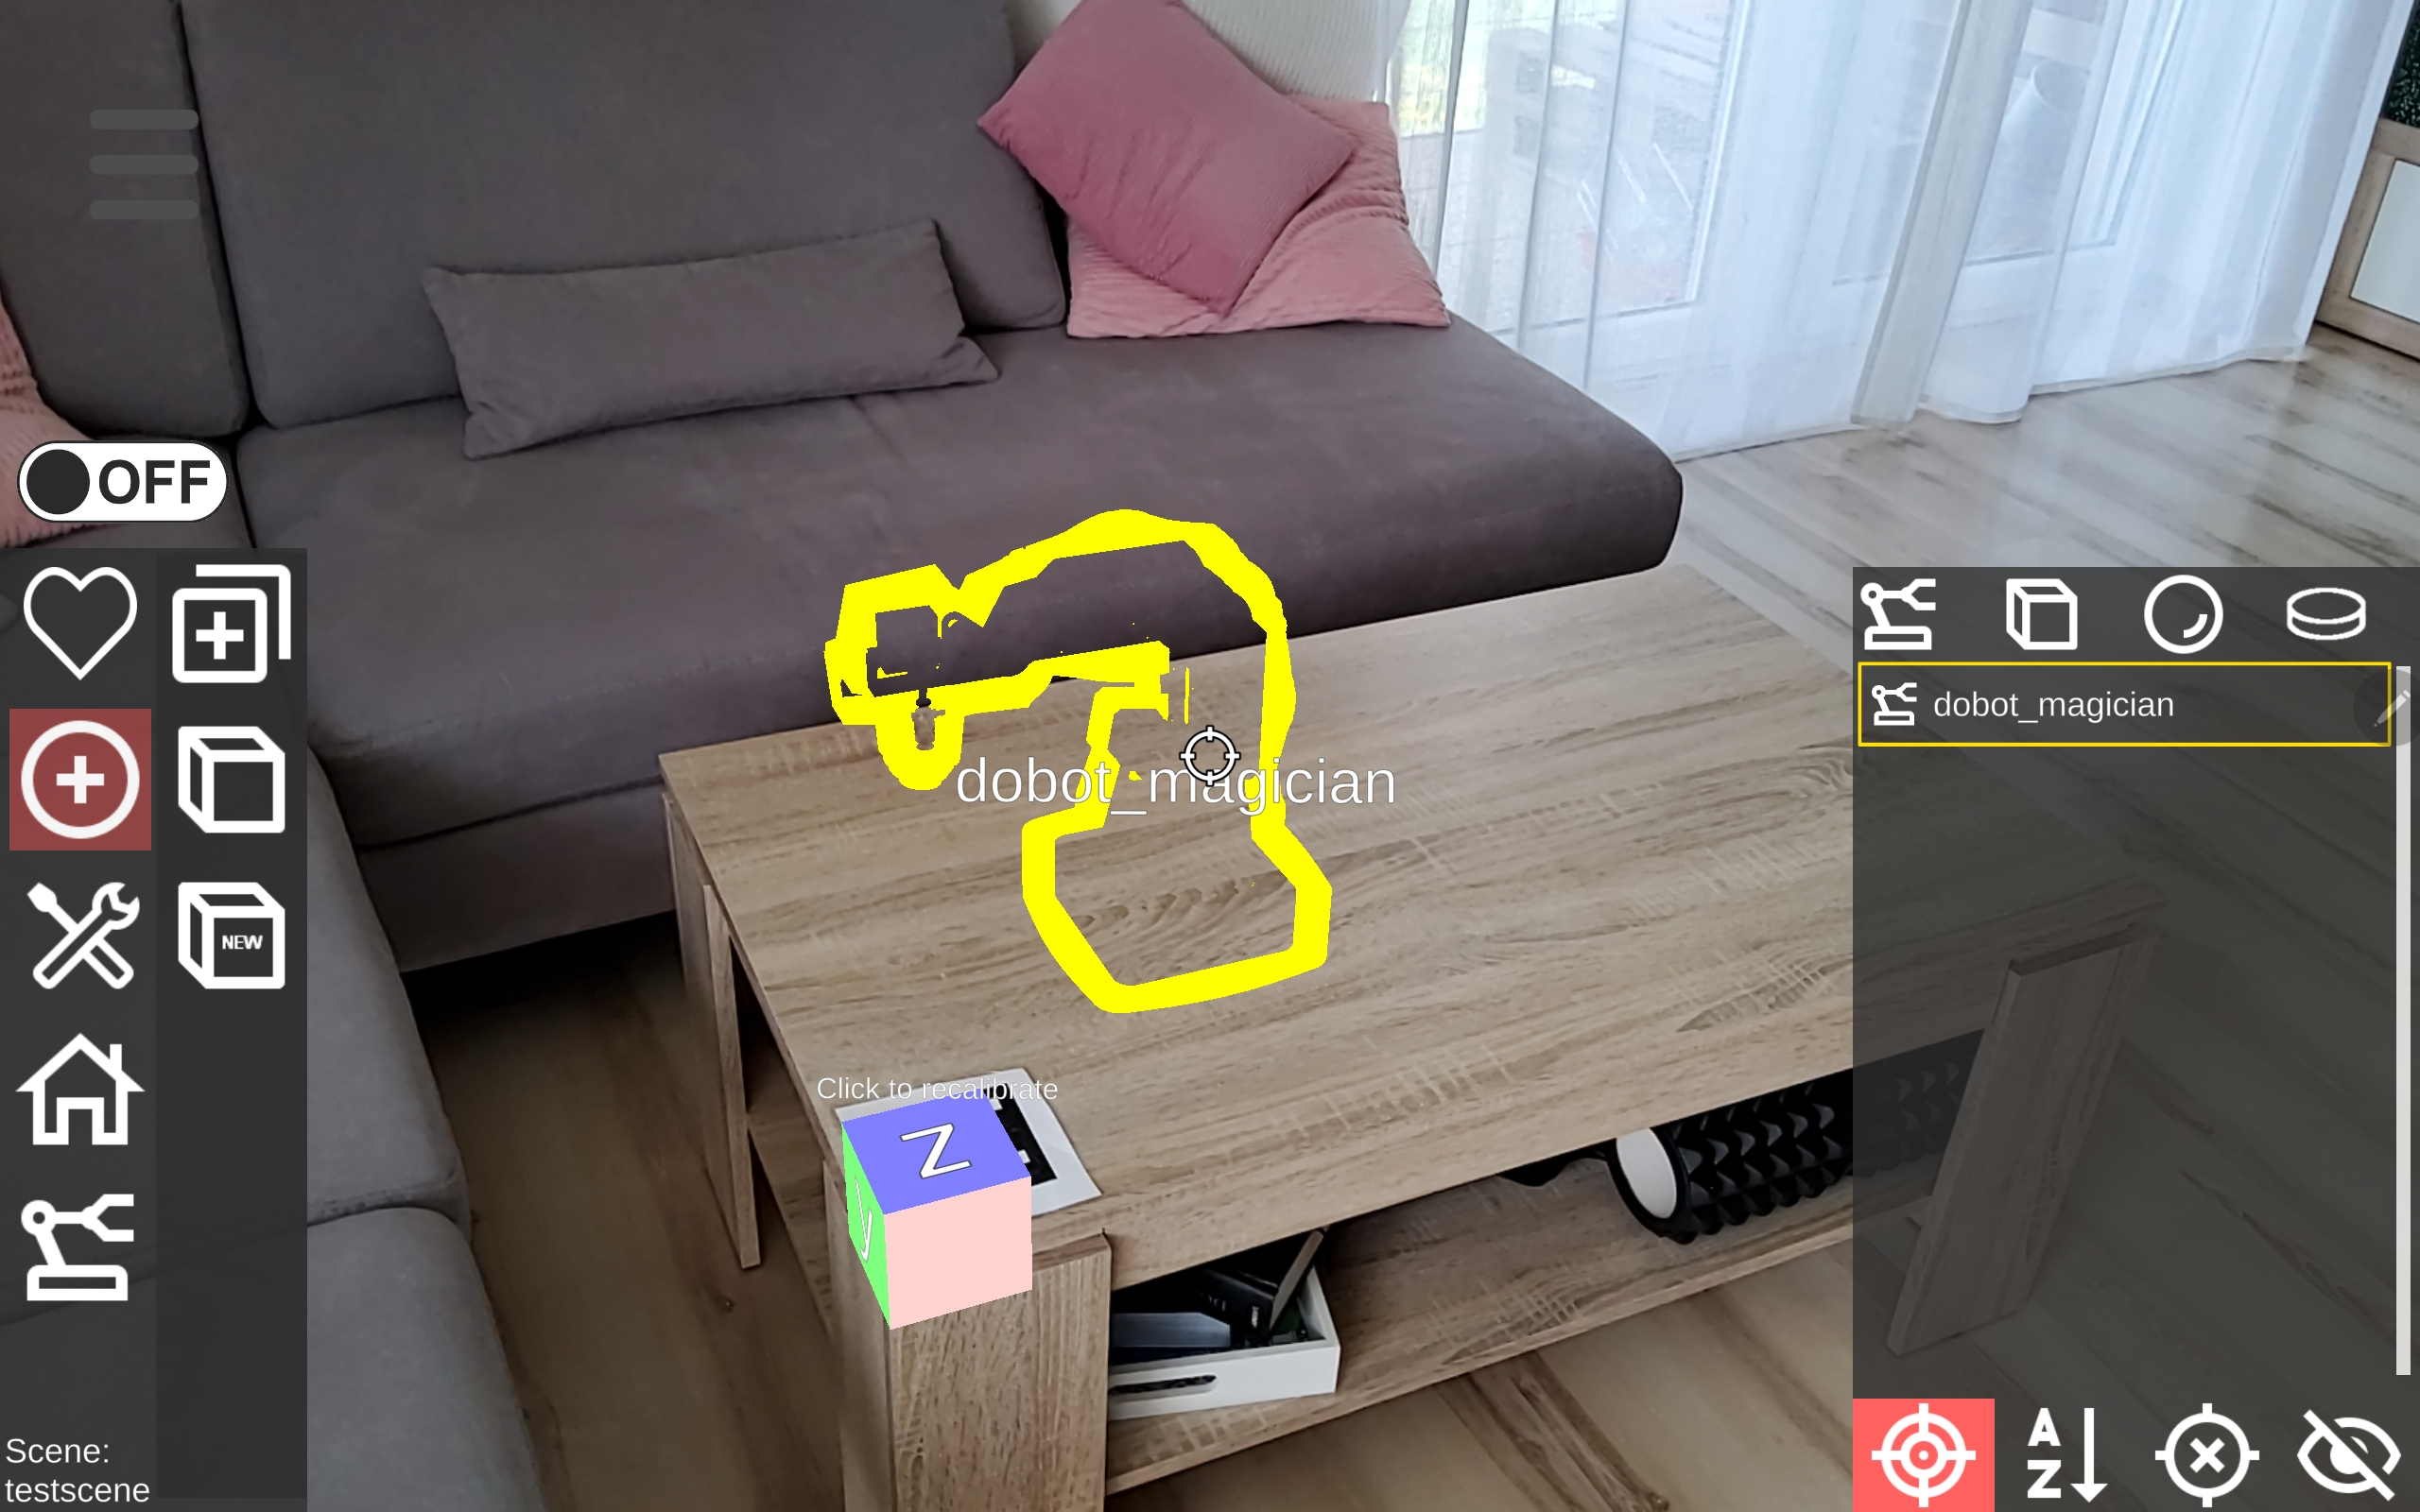
\includegraphics[width=\textwidth]{obrazky-figures/AREditorSelectorMenu.jpg}}
    
        \subfloat['Add object' menu opened.]{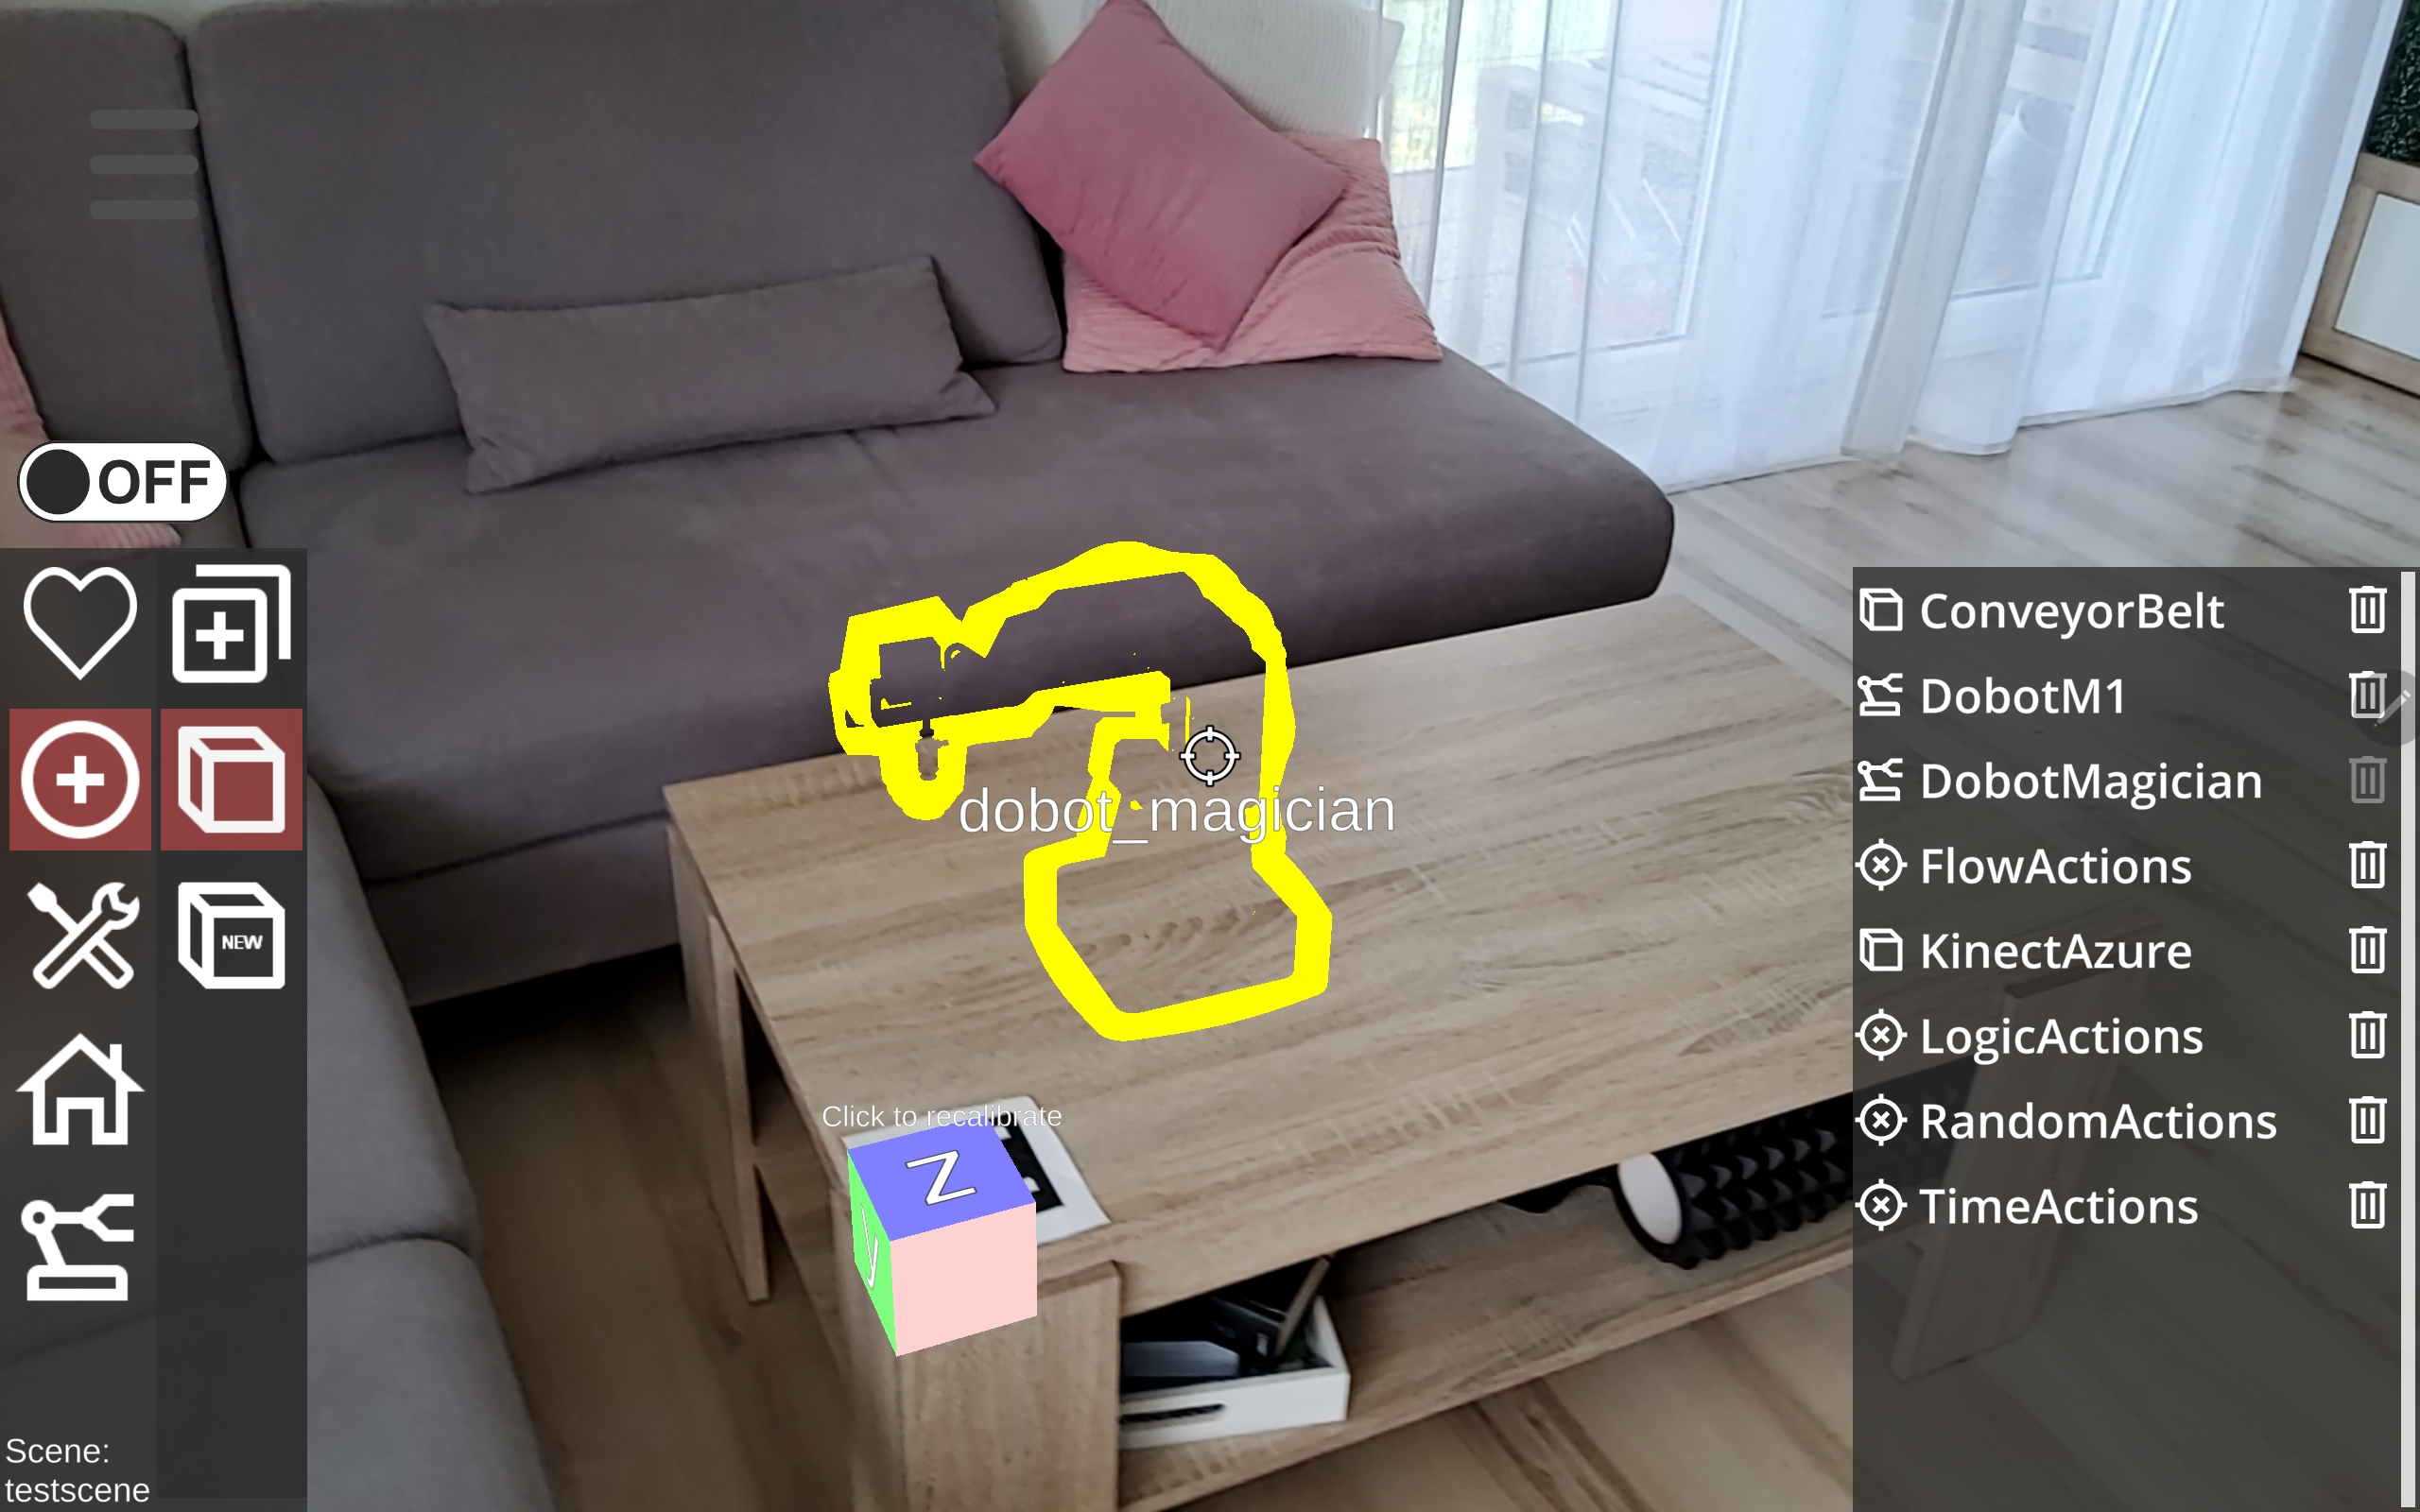
\includegraphics[width=\textwidth]{obrazky-figures/AREditorAddObjectMenu.jpg}}
    
    \caption{Editor screen}
    \label{fig:EditorMenus}
\end{figure}

The editor is designed to be used while holding a tablet with two hands. This approach introduces some limitations but helps prevent fatigue, often present when holding a tablet with a single hand for prolonged periods. Widgets are located on either side of the screen to allow for good visibility of the workspace, as well as to make the individual buttons accessible by thumbs.  

\subsubsection{3D sight}
The sight works as a de facto cursor. It is located in the middle of the screen and is the main interaction method between the user and action objects. AREditor perpetually casts a ray from the center forward and checks for collisions with action objects in the scene. By aiming the crosshair at an action object, the object is highlighted in the selector menu, as well as outlined, as seen in \ref{fig:EditorMenus}. When using the stepping menu or the object manipulation menu, the crosshair is used to select the axis of movement. 

\subsubsection{Object manipulation menu}
An action object can be moved, scaled, or rotated using the object manipulation menu. When the menu is active, a three-axis gizmo appears. By pointing the sight at a particular axis, it becomes selected, after which the transform wheel can be used to move (rotate, scale) the object along said axis. The user can also select the unit of the transform wheel, as well as move the object freely by holding the 'hand' icon and moving the tablet. The menu also offers undo and redo capabilities.


\subsubsection{Robot stepping menu}
The robot stepping menu is the main way to manually set the pose of a robot within AREditor. The appearance of the menu is similar to that of the object manipulation menu, but the transform wheel is replaced by plus and minus buttons for incremental movement. By stepping the robot, the end effector is moved in the chosen direction by the selected unit. 

The robot stepping menu also offers two more toggles, a safe/unsafe movement switch and a global/local space switch. Unlike object manipulation menu, scaling option is omitted. Both menus can be seen in \ref{manipulationandstepping}.

\begin{figure}
    \centering
    \subfloat[Object manipulation menu]{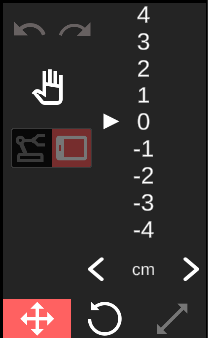
\includegraphics{obrazky-figures/objectmanipulationmenu.png}}\quad
    \subfloat[Robot stepping menu]{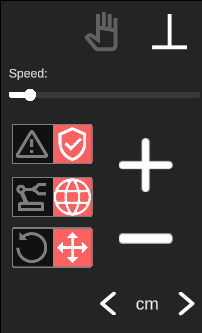
\includegraphics{obrazky-figures/robotsteppingmenu.png}}
    \caption{Object manipulation and robot stepping menus.}
    \label{manipulationandstepping}
\end{figure}

\chapter{Design}
In this chapter, I will go over the design requirements for the proposed improvement of the user interface, and the individual parts of the final design.

When programming robots using the ARCOR2 system, a user typically sets action points at the position of the end effector. An action point is a spatially anchored container, that holds a position and orientation. Actions can then be assigned to action points and program flow is created. The user, therefore, needs to be able to quickly and easily position the robot end effector to the applicable point in space so that they can set an action point. Furthermore, AREditor is designed to be used with thumbs only, warranting a simple user interface with a limited amount of buttons. 

In most previous works on mobile devices, explicit pose setting of a robot was resolved using on-screen arrows. While this approach works and was briefly considered, a better solution exists. In AREditor, selecting (and moving) objects is already done by utilizing rays cast from the camera, aimed at a chosen object within the scene. This principle can be applied to robot positioning, as described in the next section.

The goal of this design was to provide flexibility while not obscuring the screen space. This is a problem often seen in mobile AR interfaces. Another aim was to make movement feel natural and easy to learn, making it accessible to end-users of varied levels of experience with tablets or robotics.

\section{Movement}
Two approaches to robot pose setting were considered: moving individual joints, and moving the end effector only (utilizing inverse kinematics). The first approach was deemed unnecessary, as it is rarely needed. In the vast majority of use-cases, setting only the end effector position is sufficient. Secondly, as seen in \cite{Zhang2020AugmentedRI} or \cite{Tango}, this could result in a high number of buttons, obscuring the screen and complicating usage.

By shifting focus from individual joints to the end effector, the problem can be reduced to a simple point moving in 3D space, and axes can be drawn from the end effector to facilitate movement in all directions. Early designs featured arrows or joysticks on-screen to be used to move the end effector along the selected axis (\ref{fig:EarlyDesigns}).



The interface can further be simplified by utilizing tablet movement tracking. After having selected the axis, the object can be simply moved by moving the tablet. The second iteration featured a single button for axis selection and arrows (joysticks) were abandoned \ref{fig:EarlyDesigns2} \subref{SelectableAxes}. This approach also allows for unconstrained movement, which can be used by selecting the end effector itself, instead of one of the axes. This feature is available by selecting the end effector itself \ref{fig:EarlyDesigns2} \subref{SelectableEE}. Furthermore, inspired by 3D software such as Fusion 360\footnote{\href{https://www.autodesk.com/products/fusion-360/}{https://www.autodesk.com/products/fusion-360/}} or Godot Engine\footnote{\href{https://godotengine.org/}{https://godotengine.org/}}, the gizmo was modified to include planes, which allow unconstrained movement in a 2-dimensional space. 

\begin{figure}[H]
    \centering
        \subfloat[Design with two sets of joysticks, to control all three axes.]{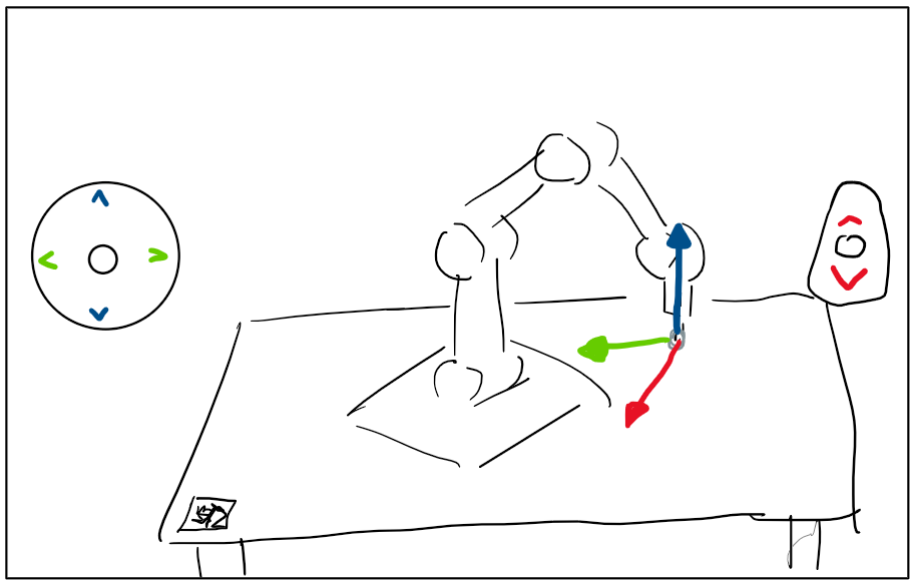
\includegraphics[width=0.8\textwidth]{obrazky-figures/EarlyDesign2.png}
        \label{EarlyDesign2}}
    
        \subfloat[Arrows replace joysticks, and a dial to set the gizmo rotation.]{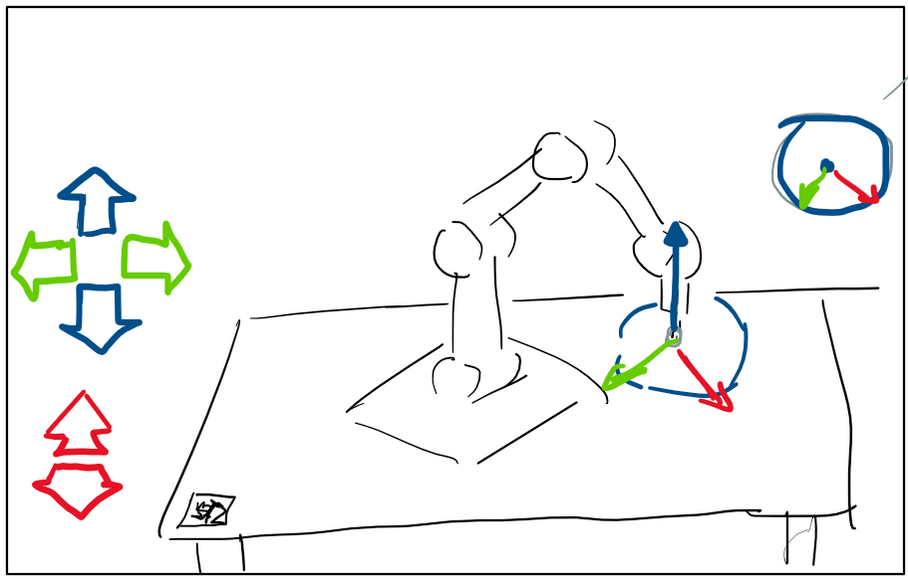
\includegraphics[width=0.8\textwidth]{obrazky-figures/EarlyDesign1.png}
        \label{EarlyDesign1}}
    
    \caption{Early designs with on-screen touch controls}
    \label{fig:EarlyDesigns}
\end{figure}

\begin{figure}[H]
    \centering
        \subfloat[Selectable axes]
        {
        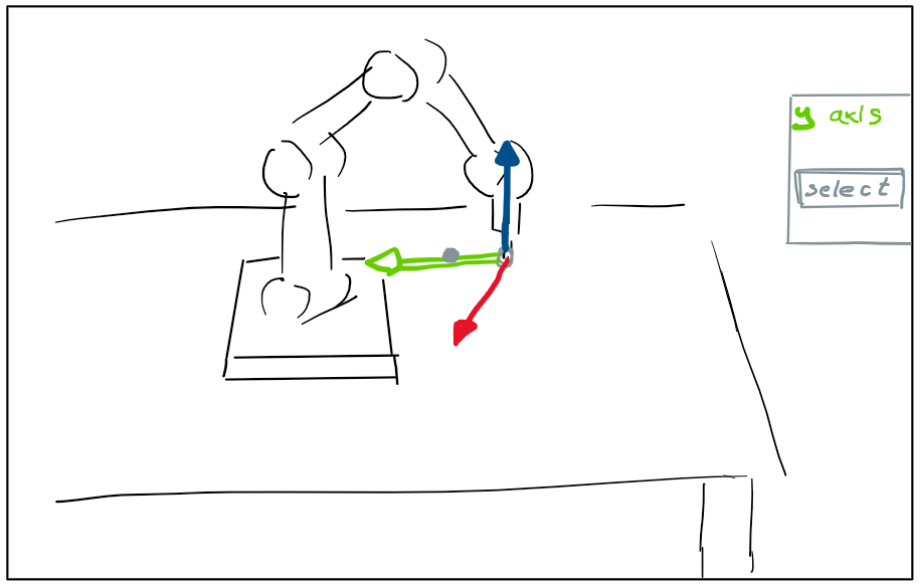
\includegraphics[width=0.8\textwidth]{obrazky-figures/EarlyDesign3.png}
        \label{SelectableAxes}
        }
    
        \subfloat[Selectable end effector]{
        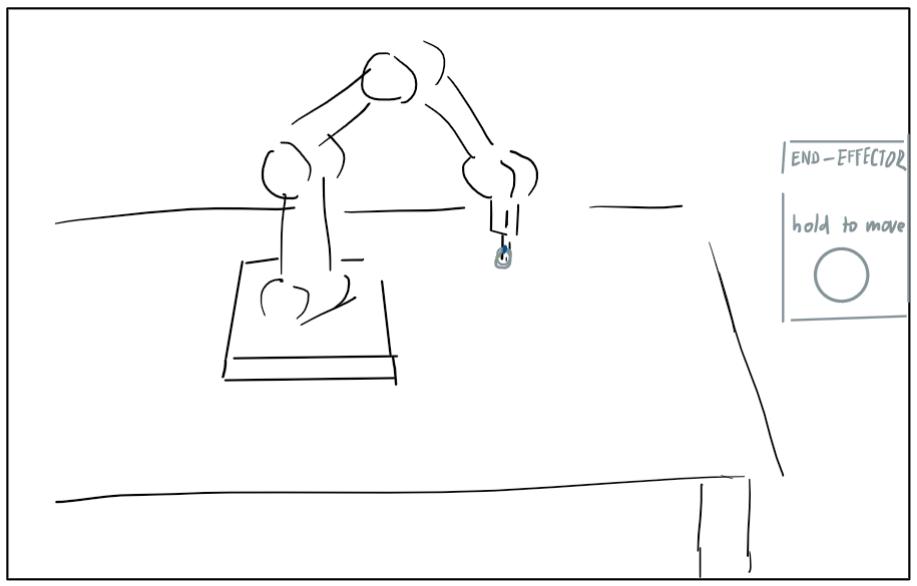
\includegraphics[width=0.8\textwidth]{obrazky-figures/EarlyDesign4.png}
        \label{SelectableEE}
        }
    
    \caption{Design variants employing tablet movement. These were later combined into singular design.}
    \label{fig:EarlyDesigns2}
\end{figure}

\subsection{Forward/backward buttons}

To facilitate movement in the direction from the user to the robot, an additional control was added. To move the end effector forward, one would have to move the tablet forward the same amount, which proved to be impractical. In order to allow the operator to keep the same distance from the robot throughout the session, a different way to move the end effector along said axis was necessary. A dual button control was added, featuring slanted arrow icons to illustrate the forward/backward direction of movement (\ref{fig:forwardbackwardbuttons}). 

These buttons were later modified to only affect the horizontal plane, ignoring the vertical axis. This was decided after a consultation, where it was deemed to be the more logical approach. The buttons were added to remove the need to walk forward and backward, regardless of the height of the user. \myworries{add a picture perhaps}
\\
\begin{figure}[H]
    \centering
    
\includegraphics{obrazky-figures/forwardbackwardbuttons.png}
    \caption{Forward/backward buttons.}
    \label{fig:forwardbackwardbuttons}
\end{figure}

\subsection{Sensitivity sliders}

When dragging the end effector, the end effector position moves to the exact position of the raycast at a specified distance. This is the most intuitive outcome, but positioning the end effector with high precision can be cumbersome. By introducing variable sensitivity, the user can modify the ratio of tablet movement to end effector movement, and thus make more precise adjustments easier. 

Another issue is distance. When standing farther away, the same tablet movement results in a larger robot movement. For example, when standing 1.5 meters away and rotating the tablet by 15\degree, while having the X axis selected, the end effector will move by 40 centimeters. If the operator stood a meter farther, the end effector would move by 66 centimeters \ref{fig:closefar}. Having adjustable sensitivity can therefore be useful in scenarios, where the operator has to stand far away. The slider value acts as a distance multiplier and is by default set to 1, which moves the end effector to the exact final raycast hit and can be lowered to shorten the distance traveled by the robot arm. 

Similarly, a slider for the forward/backward buttons was added, to control the speed of the movement. 

\begin{figure}
    \centering
    \subfloat{
        \includesvg[width=0.3\textwidth]{obrazky-figures/dobotmagician.svg}
        \label{close}
    }
    \qquad
    \subfloat{
        \includesvg[width=0.3\textwidth]{obrazky-figures/dobotmagicianfar2.svg}
        \label{far}
    }
    
    \caption{The same tablet rotation from different distances.}
    \label{fig:closefar}
\end{figure}

\subsection{User-relative coordinate system}

To allow the user to move the end effector along an arbitrary axis in the horizontal plane, two approaches were examined. Initially, a dial for manually rotating the gizmo around its vertical axis was considered (\ref{fig:EarlyDesigns}\subref{EarlyDesign1}). A more intuitive approach is to make the gizmo rotation relative to the tablet position. In this scenario, the gizmo rotates as the user moves around the workplace, with one axis staying perpendicular to the camera position and the second one oriented towards the camera position \myworries{pic}. Another addition is a lock button, which allows the operator to lock the current gizmo rotation. This system enables movement along arbitrary axes, which can be aligned with other objects in the workplace by simply walking toward them while maintaining the repeatability of movements provided by the lock button. 

\section{User interface}
The system consists of several separate submenus: the main menu, forward/backward buttons, and a confirmation dialog.

The main menu's central component is the select button. It also contains a label indicating the current selection, a sensitivity slider, and the coordinate system switch. The select button has a description label "hold to drag", which gets hidden when dragging. The coordinate system switch has two switchable states, \textit{world} and \textit{user}, through which the user-relative coordinate system can be enabled. When the \textit{user} state is selected, the lock button appears. 

The layout follows previously established conventions in AREditor. The main menu is located on the right side of the screen, with the confirmation dialog beneath. The main menu is always visible, the other menus are turned on and off when required. If the pose of the robot model is the same as the real robot, the confirmation dialog is not visible. It only appears, when a movement robot model is executed, and is only enabled, when the user concludes the movement. The confirmation dialog contains two buttons, \textit{apply} and \textit{revert}, through which the operator can send the pose to be applied to the real robot, or revert the model to the default state (copy the pose of the real robot). Additionally, while dragging, the left menu along with the online/offline switch are hidden. The layout of the menus can be seen in \ref{fig:layout}.

\begin{figure}
    \centering
    \subfloat[The layout when not moving.]{
        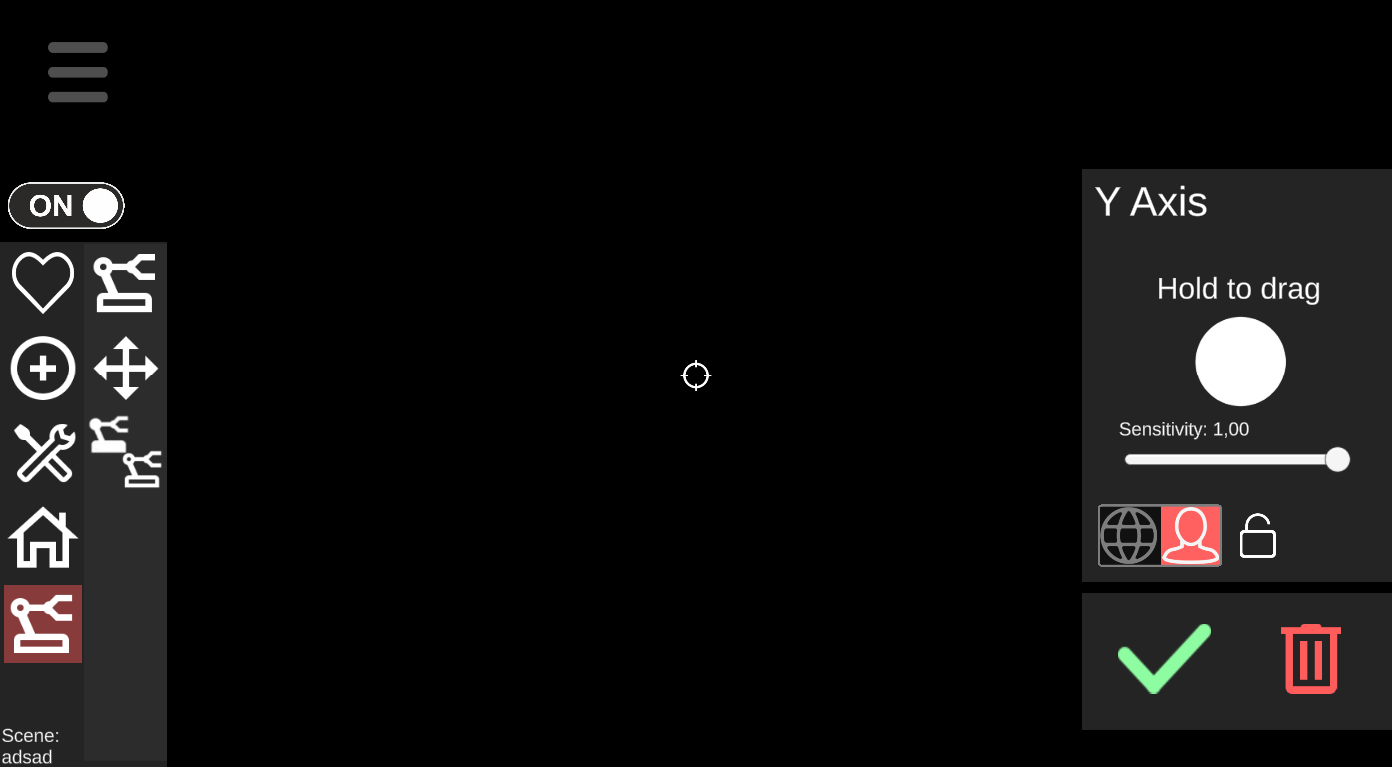
\includegraphics[width=0.8\textwidth]{obrazky-figures/Layout.png}
        \label{notmoving}
    }
    \\
    \subfloat[The layout when moving the end effector.]{
        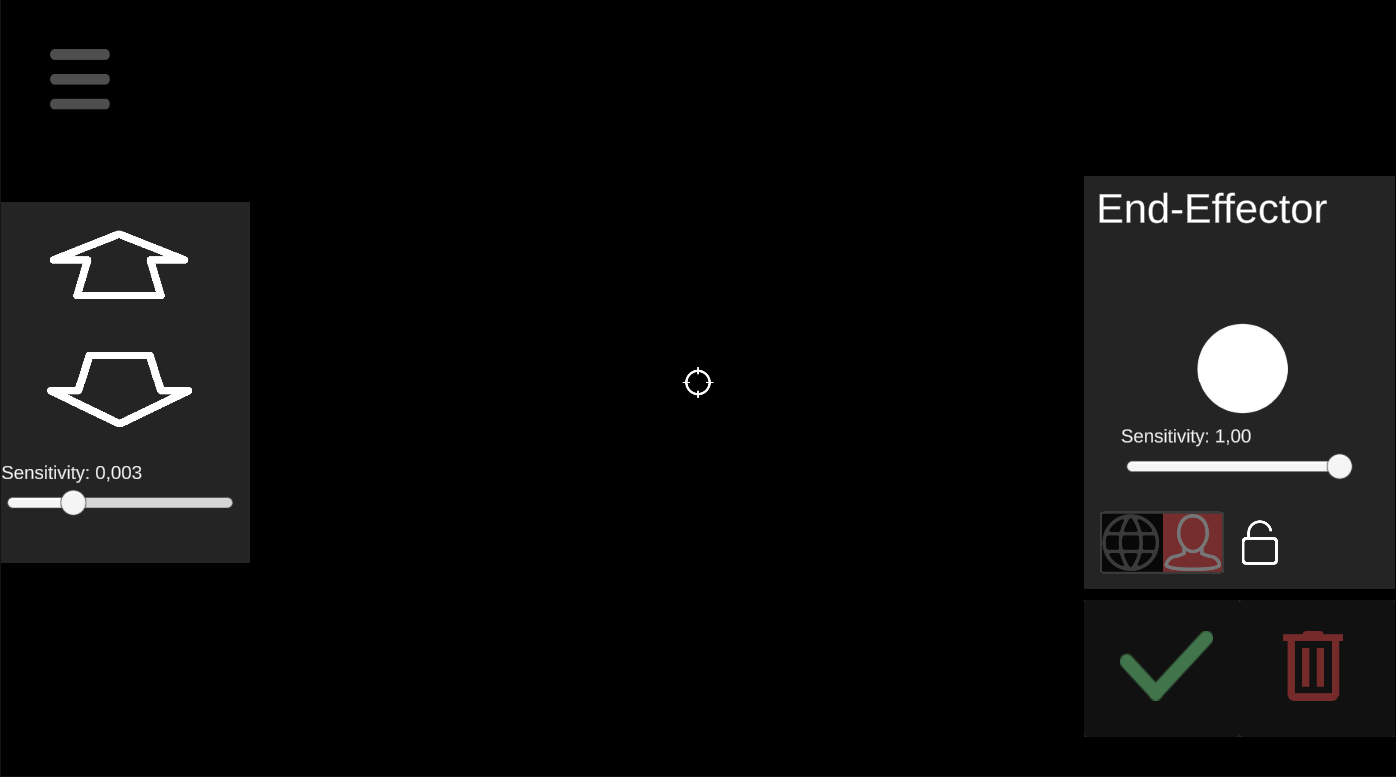
\includegraphics[width=0.8\textwidth]{obrazky-figures/LayoutWhenMoving.png}
        \label{moving}
    }
    
    \caption{A comparison of the old notification and the new notification. \myworries{replace with drawings}}
    \label{fig:layout}
\end{figure}

\subsection{Invalid pose indication} 

To inform the user that the pose is out of bounds, visual indicators were included in the design. The original notification system was insufficient for the purposes of this solution for two reasons: readability and performance, the first of which will be characterized in this section. Performance is discussed in the \textit{Implementation} chapter.

Notifications in the original notification system are implemented as temporary messages in the top right corner of the screen. A notification is presented in the form of a semi-transparent grey box, which contains text. If the notification informs of a failed RPC request, it usually contains a title and the error message from ARServer. The notification fades in, is displayed for a brief period, and then fades out. 

This work entails a different form of notification. The user has to be notified exactly when an impossible pose is reached, and vice versa, when the point is back in a valid position, for quicker understanding of the current state. The message should also be simpler, as there is no need to display the full RPC response message.

The new notification is a red box, containing the text "Invalid pose" written in large, white text. The RPC response message was removed. It appears immediately after the user moves the end effector beyond the reach of the robot, and is hidden once the end effector is back in the work envelope of the robot arm. A comparison between the old and the new notifications can be seen in \ref{fig:notifications}.

\begin{figure}[h]
    \centering
    \subfloat[The old notification.]{
        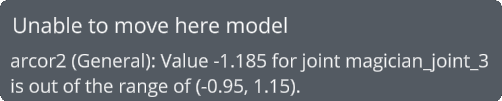
\includegraphics{obrazky-figures/OldNotification.png}
        \label{old}
    }
    \\
    \subfloat[The new notification.]{
        
\includegraphics{obrazky-figures/ImpossiblePoseNotification.png}
        \label{new}
    }
    
    \caption{A comparison of the old notification and the new notification.}
    \label{fig:notifications}
\end{figure}

An additional visual cue was added to further indicate, that the robot is in an unreachable pose. Upon leaving the work envelope, the robot model is displayed in red \myworries{img}. A more elaborate, albeit similar approach was taken in \cite{ONG2020101820}, where the overlaid robot model arm is displayed in colors from green to red, based on the manipulability of the robot. The system calculates manipulability based on a scale proposed by Yoshikawa \cite{yoshikawa}. In the ARCOR2 system, no such manipulability scale is implemented and is out of the scope of this work, therefore a simpler, yet still effective, approach was chosen.

\chapter{Implementation}

The system was integrated into AREditor as a new menu in the 'Robot' category. The main part of the solution is the \texttt{ModelSteppingMenu} controller. 

\section{Unity\myworries{?}}

\section{Movement}

Upon opening the menu, a 3D gizmo is instantiated in the position of the end effector. Each of the gizmo's axes and planes, as well as the center point of the gizmo, serve as a handle, which can be selected and dragged by moving the tablet. Raycasting is utilized to track the tablet's movement in space:

\begin{enumerate}
    \item When the user initiates dragging, a ray is cast from the screen's center and a point along the ray is recorded at a specified distance (\texttt{originalPosition}).
    \item During every frame while dragging, a new ray is cast and the \texttt{targetPosition} is recorded in the same way.
    \item The difference between \texttt{originalPosition} and \texttt{targetPosition} serves as the translation vector.
\end{enumerate}

Calculating the difference between points along rays forms the basis of movement. When the user presses and holds the select button initiating movement, a ray is cast from the middle of the screen, and a point along said ray at a specified distance (\texttt{pointDistance}) is recorded. This point represents the original position before translation. The target position is set during every frame by casting a ray and retrieving a point similarly. The difference between these two points serves as the translation vector.

The original point position has to be set this way for two reasons. Firstly, the ray cast in the current frame might not be colliding with the selected axis at the time of initiating movement, because the might have been selected earlier. An axis stays selected, even when no ray is colliding with it, and only gets deselected once a different axis is targeted instead. If the original point position were set to the position of the last collision, the gizmo would snap into position, as the starting position would not be exactly where the camera is currently facing. By defining the original position as a point along a ray in the current frame, the starting point of the translation is in the exact spot the camera is presently facing, eliminating initial snapping to position. \texttt{pointDistance} is set at an earlier instance when the axis is initially selected, which results in an imprecise distance measurement, but the inaccuracy is not noticeable. In \ref{fig:movementdemo}, a visual description of how a movement is projected onto an axis can be found.

\begin{figure}[h]
    \centering
    \subfloat[At 1.00 sensitivity.]{
        \includesvg[width=0.4\textwidth]{obrazky-figures/movementdemostration.svg}
        \label{full}
    }
    \qquad
    \subfloat[At 0.80 sensitivity]{
        \includesvg[width=0.4\textwidth]{obrazky-figures/movementdemostrationlowsens.svg}
        \label{eighty}
    }
    
    \caption{An illustration of movement along the X-axis. a) original point position, b) target point position, c) final end effector position.}
    \label{fig:movementdemo}
\end{figure}

The translation is first applied to a dummy \texttt{GameObject}. Creating an empty GameObject is necessary because Unity only allows Transforms to be instanced along with a GameObject. The dummy's transform is reset at the beginning of every frame; the position is set to the original point position pre-translation, and the rotation is set to the draggable point's rotation. Using the Unity method \texttt{Transform.Translate()}, the translation is applied, either unconstrained or only on selected axis/axes. By using the \texttt{Translate} method, the translation is applied relative to the object's local axes, taking the current rotation of the gizmo into account. The translation vector is also transformed into the local space of the point using \texttt{Transform.InverseTransformVector()}. 

Forward/backward buttons' functionality is facilitated by moving the target point position in world space. During every frame, if either the forward or backward button is held, the direction vector from the camera to the target point is normalized, multiplied by the current sensitivity multiplier, and added to a \texttt{Vector3} variable, \texttt{forwardBackwardAdjust}. The value's \texttt{x} and \texttt{z} coordinates are added to the target point position to constrain the movement to the horizontal plane. The variable is reset when the movement is completed. 

Calculating the inverse kinematics for a given point, which is represented with a \texttt{Vector3}, involves three steps:
\begin{enumerate}
    \item The point is transformed from world space to the local space of the scene.  
    \item The point is converted from Unity coordinate system to ROS coordinate system.
    \item A \texttt{Position} is created from the Vector3 representation, which casts the float values to decimal.
\end{enumerate}

\section{Gizmo}

The 3D gizmo used in this system is a variant\footnote{\href{https://docs.unity3d.com/Manual/PrefabVariants.html}{https://docs.unity3d.com/Manual/PrefabVariants.html}} of the gizmo prefab used in other menus, such as \texttt{RobotSteppingMenu}. The gizmo was modified by removing distance labels and adding planes, as well as a custom controller, \texttt{GizmoVariant}, which provides helper methods for highlighting planes and axes, as well as flipping the gizmo around the X, Y, and Z axes. Upon opening the menu, the gizmo is instantiated as a child of \texttt{DraggablePoint}, which represents the end effector and is used as a handle for dragging in all three axes.

When an axis (plane, point) is selected, the movement can be initiated by pressing and holding the main button. All unselected axes and planes are gradually hidden by manipulating their scale, and the selected axis is lengthened. A coroutine was used to gradually change the scale of a chosen axis across several frames\footnote{\href{https://docs.unity3d.com/Manual/Coroutines.html}{https://docs.unity3d.com/Manual/Coroutines.html}}. The advantage of using a coroutine is that they can be started and stopped, instead of always checking the state every frame. This makes them better suited for infrequent tasks, such as scaling the axes upon initiating movement. Another benefit is cleaner code in the \texttt{Update} method.

\begin{lstlisting}[style=sharpc, breaklines=true]

//the parameter "scale" is the target scale of the axis
private IEnumerator AxisScale(GameObject axis, Vector3 scale) {

    //coroutine is concluded once the scale is within a threshold
    while (Vector3.Distance(axis.transform.localScale, scale) > 0.01f) {
    
        //linear interpolation is used to smooth the animation
        axis.transform.localScale = Vector3.Lerp(axis.transform.localScale, scale, 0.25f);

        //return control to Unity, and continue in the next frame
        yield return null;
    }

    //after the threshold is crossed, the final scale is applied directly
    axis.transform.localScale = scale;
}
\end{lstlisting}

\myworries{add images of gizmo here}

The typical use case is that of a user walking freely in the workspace, looking at the robot from different sides. To allow easy access from all sides, the gizmo is flipped on the corresponding axis, if the camera moves across it. This is done by transforming the position of the camera from world space into local space of the \texttt{DraggablePoint} using the Unity method \texttt{Transform.InverseTransformPoint()} and checking the coordinates for positive/negative values. The flip itself is achieved by simply multiplying the chosen coordinate value by -1.

When the user-relative coordinate system is enabled, the gizmo's X-axis always faces the camera. The Unity method \texttt{Transform.LookAt()} was used, and the rotation was limited by modifying the target's Y-coordinate:\footnote{\href{https://discussions.unity.com/t/lookat-to-only-rotate-on-y-axis-how/10895/3}{https://discussions.unity.com/t/lookat-to-only-rotate-on-y-axis-how/10895/3}}

\begin{lstlisting}[style=sharpc, breaklines=true]
    //Y coordinate set to self to constrain rotation
    Vector3 targetPosition = new Vector3(
        Camera.main.transform.position.x,
        pointInstance.transform.position.y,
        Camera.main.transform.position.z
        );
        
    pointInstance.transform.LookAt(targetPosition);

\end{lstlisting}

\section{Clipping shader}

When a plane is selected as a form of movement, it needs to be visually indicated. An approach that was initially tested was stretching the plane, analogous to the way axes are elongated when selected. The idea was, that the plane would cut through the middle of the robot, visualizing its position in relation to the robot in space. Due to how rendering works, however, this is not easily achievable. Either the robot or the plane will always be rendered on top. The solution to this problem is a custom shader.

When enabled, the clipping shader is assigned to the material of the robot renderer. A \texttt{float4} property \texttt{\_Plane} represents the clipping plane in the shader. The first three values are the normal of the plane, and the fourth is the distance to the origin, along the plane's normal. In the surface shader, the dot product of the surface point's world position and the plane position is calculated. The fourth value is added to account for the distance of the plane from the origin. If the result is positive, the point is above the plane, if the result is zero, the point lies directly on the plane, and if the result is negative, the point is below the plane. All the points below the plane have an alternate color added to their base color.

\begin{lstlisting}[style=sharpc, breaklines=true]
void surf (Input i, inout SurfaceOutputStandard o) {
    //dot product is evaluated
    float distance = dot(i.worldPos, _Plane.xyz);

    //distance from origin is added
    distance = distance + _Plane.w;

    //point is above the plane, render normally
    if (distance > 0) {
        fixed4 col = tex2D(_MainTex, i.uv_MainTex);
        col *= _Color;
        o.Albedo = col.rgb;
    
    //point is below the plane, add tint
    } else {
        fixed4 col = tex2D(_MainTex, i.uv_MainTex);
        col *= _Color;
        o.Albedo = col.rgb + _AlternateColor.rgb;
    }
}
\end{lstlisting}

The clipping plane property is set from the \texttt{ClippingPlane.cs} script, which is attached to an empty \texttt{GameObject} and inherits the gizmo's \texttt{Transform}. The clipping plane holds a list of materials with the clipping shader assigned. Materials are added and removed from the list to enable and disable the shader during runtime. In each frame, the script creates a new plane, loops through the material list, and sets the \texttt{\_Plane} property in the shader. The method was adapted from \footnote{\href{https://www.ronja-tutorials.com/post/021-plane-clipping/}{https://www.ronja-tutorials.com/post/021-plane-clipping/}} and \footnote{\href{https://www.youtube.com/watch?v=shOH7pJSxk8}{https://www.youtube.com/watch?v=shOH7pJSxk8}}.

\begin{lstlisting}[style=sharpc, breaklines=true]
void Update() {
    //create plane
    Plane plane;
  
    plane = new Plane(transform.up, transform.position);
    
    //transfer values from plane to vector4
    Vector4 planeRepresentation = new Vector4(plane.normal.x, plane.normal.y, plane.normal.z, plane.distance);
    
    //pass vector to shaders
    foreach (Material material in Materials) {
        material.SetVector("_Plane", planeRepresentation);
    }
    
}
\end{lstlisting}

\myworries{add pictures of shader}

This creates a horizontal plane at the position of the gizmo. There are, however, three planes that can be selected. In order to properly split the model when a different plane is used, the \texttt{ClippingPlane} object is rotated accordingly. Another aspect to consider is the camera's location in reference to the gizmo; if not accounted for, it would result in the colors being switched (red in front of the plane, regular behind it).

This approach to visualizing the plane was abandoned in later development. While the effect worked well, the stretched plane covering much of the workspace was deemed too irritating. A more elegant approach was used to indicate, which plane the movement is constrained to: instead of stretching the plane itself, the two axes that define the plane are elongated. This method is more elegant, as it uses visual elements the user is already familiar with, instead of introducing new ones. 


\section{Invalid pose indication}


\subsection{Notifications}

Severe performance issues were noted during development when dragging the point out of bounds. The notifications were identified as the root cause. Each notification is an instance of \texttt{NotificationEntry}, created by the singleton \texttt{Notifications}. The lifespan of each instance is tied to a timer. When dragging the robot arm, an inverse kinematics request is sent to ARServer nearly every frame. If the operator moves the target point outside the work envelope of the robot, the RPC fails, and an RPC response informing of failure is sent. AREditor creates a notification for each of these responses. This essentially floods the app with notifications and results in severe lag, sometimes causing the tablet to freeze for tens of seconds at a time. 

The new notification is a single GameObject already instantiated within the \texttt{ModelSteppingMenu} and its state is switched between active and inactive based on the current target point position and therefore pose validity. 

\subsection{Robot display}

When the target point is unreachable, the robot turns red. This was implemented with a surface shader in the file \texttt{InvalidPose.shader}. The red color is added to the base color, which tints the robot red while preserving the original texture:

\begin{lstlisting}[style=sharpc]

void surf (Input IN, inout SurfaceOutputStandard o)
{
    //main color is obtained from the main texture
    fixed4 c = tex2D (_MainTex, IN.uv_MainTex) * _Color;
    //red color is added
    o.Albedo = c.rgb + _RedColor.rgb;
}
\end{lstlisting}

The shader is applied to the materials of the robot renderers at runtime. A robot renderer contains three materials when the outline is enabled: mask, object material, and outline. If the outline is disabled, only the object material is present. The following code snippet illustrates how the red shader is enabled (adapted from a function for setting visibility in  \texttt{RobotActionObject}). Disabling the shader is done by applying the 'Standard' shader, which is done correspondingly.

\begin{lstlisting}[style=sharpc]

private void EnableInvalidShader() {
    materialEnabled = MaterialEnabled.invalid;
    foreach (Renderer i in robot.robotRenderers) {
        if (i.materials.Length == 3) {
            i.materials[1].shader = Shader.Find("InvalidPose");
        } else {
            i.material.shader = Shader.Find("InvalidPose");
        }
    }
}
\end{lstlisting}

\myworries{put an image of the red robot here}

\chapter{Usability testing}

Testing took place in the robotics laboratory at FIT. Due to scheduling conflicts, the testers were split into two groups of 3 and 2, and the testing was done in two separate sessions. The test subjects were students of the third year at BUT FIT. 

The test subjects were first asked questions to assess their level of experience with tablets, AR, and robotics. All subjects shared a moderate level of experience with tablets and a low to moderate level of experience with AR, but none have come in contact with robot programming. As the solution is targeted towards end-users with no experience with robotics, this makes the subject group ideal for usability testing. The general outline of the testing consisted of several points:

\begin{itemize}
    \item Ask questions about experience, briefly explain, what AREditor is for
    \item Present the subject with the application, observe initial instincts
    \item Explain, how the model stepping menu generally works, notice how quickly the subject picks it up
    \item Gradually explain all the features of the menu
    \item Present simple tasks to the subject
    \item Show the subject the robot stepping menu
    \item Ask them to compare the two menus
    \item Conclude testing, ask for any additional feedback
\end{itemize}

Subjects were also encouraged to ask questions and give feedback throughout the entire testing.

\section*{Subject 1}

The first subject initially assumed, that the select button worked like a joystick and attempted to use it as such (pulling to the sides when holding it down). However, after explaining how the menu is supposed to be used, they picked it up within seconds. 

The subject was able to accomplish simple tasks such as positioning the robot to the given coordination and moving the end effector along a global axis. When tasked with moving the end effector along the edge of the table which is not aligned with the global coordinate system, the subject enabled the user-relative coordinate system, aligned themselves with the table, and moved the robot using the correct axis. The subject correctly assumed the purpose of the 'Apply pose' and 'Revert pose' buttons. 

After reviewing the robot stepping menu, the subject concluded, that the new solution is a significant improvement. They especially liked the ability to simply drag the model into a pose and visualize it, in contrast with the robot stepper, where they could not easily tell where the robot arm would end up before pressing a button.

The subject struggled when they stopped moving the point while out of reach of the robot. They did not know, what to do. The subject also suggested labeling the sensitivity slider, and assessed, that before using a plane for movement, they couldn't tell, what it was for, although that was apparent once they selected it for the first time. When it comes to the clipping shader, the subject failed to notice it, and when brought up, they were unsure of its purpose.

\section*{Subject 2}

When tasked with moving the robot arm to a designated location, without any prior explanation of how the system works, the second subject successfully did so. Given the task of moving the robot arm along an arbitrary axis, the subject correctly assessed, that the user-relative coordinate system should be enabled, but then they selected the horizontal plane instead of the Y-Axis on accident. The subject also correctly assumed the purpose of the forward/backward buttons, but the sensitivity range was too high, making it impractical to use. This was amended before further testing.

When using the robot stepping menu, the subject also found it hard to predict, where the end effector would end up, and preferred the model stepping menu due to its transparency. 

The second subject, just like the first subject, suggested labeling the sensitivity sliders. They also found it frustrating when going out of bounds and having to find the way back, partly due to having no sense of depth. The clipping shader served no purpose other than a source of confusion in this testing too.

\section*{Subject 3}

The third subject initially attempted to drag the gizmo arrows with their finger on-screen, but quickly caught on. When tasked with moving the point along the axis of the table, the subject correctly utilized the user-relative coordinate system, aligned themselves with the edge of the table, and proceeded to move the point along the right axis. They also correctly understood the functionality of the planes. In comparison with the robot stepping menu, the model stepping menu was deemed far more user-friendly.

Various times during the testing, when attempting to move the point across the robot itself, the subject stopped and backtracked, if the robot turned red. This suggests, that the subject also struggles to interpret, where the point is in relation to the robot while out of bounds. As with the previous subjects, the clipping shader also went unnoticed and misunderstood.

\section*{Subjects 4 and 5}

On the second day of testing, the tasks were slightly modified to better reflect real-life scenarios. Colored cubes were used as targets, and the subjects' job was to move the end effector towards them. 

The fourth and fifth subjects came in at the same time and tested alternately. The fourth subject attempted to move the gizmo using their finger, analogous to subject 3, but very quickly realized how it worked.
As the fifth subject was present during this time, their first instinct could not be observed. They both understood the purpose of the user-relative coordinate system, and they utilized the forward/backward buttons during various tasks. 

One thing that subjects 4 and 5 did differently was utilize the robot stepping menu. While they agreed that it is tedious to use for large movements, it can be useful for precise adjustments. When tasked with aligning the end effector with a cube, they often opted for a workflow that included both the model stepping menu and the robot stepping menu.

\section{Evaluation}

In total, 5 people over 2 days tested the application. They all concluded, that the model stepping menu is an improvement over the robot stepping menu in terms of usability, speed, and transparency. Below is shown a table with the testing results. 

\begin{table}[h!]
    \centering
    \begin{tabular}{|p{0.2\linewidth}|p{0.12\linewidth}|p{0.12\linewidth}|p{0.12\linewidth}|p{0.12\linewidth}|p{0.12\linewidth}|}
         \hline
         & 1 & 2 & 3 & 4 & 5   \\
         
         \hline
         \textbf{Principle grasp} & fast & immediate & fast & very fast & very fast \\
         
         \hline
         \textbf{Movement choice} & EE, axes & EE, planes & EE, axes & Axes, EE & EE, axes \\

         \hline
         \textbf{Movement issues} & no issues & misselected axis & no issues & misselected axis & no issues \\

         \hline
         \textbf{User-relative coord. system usage} & yes & yes & yes & yes & yes \\
         
         \hline
         \textbf{FW/BW buttons usage} & no & no & occasionally & often & occasionally \\
         
         \hline
         \textbf{Sensitivity change} & no & yes & yes & yes & no \\

         \hline
         \textbf{Robot stepping menu usage} & no & no & no & yes & yes \\

         \hline
         \textbf{Clipping shader understanding} & no & no & no & no & no \\
         
         \hline
         
    \end{tabular}
    \caption{Usability testing evaluation}
    \label{tab:testing}
\end{table}

This testing yields several key insights. Firstly, most subjects naturally gravitated towards the end effector as their initial choice of movement mode. Axes saw more use as each session progressed, showing that they are better suited for tasks requiring a level of precision, but they are not as intuitive to use at first. Axes were most often used in combination with the user-relative coordinate system. The planes were used sparsely throughout the testing, and occasionally they were selected accidentally. Consequently, the planes were made smaller and were moved further away from the axes to prevent any future incidents of similar nature. 

The forward/backward buttons saw moderate use, the problem was the sensitivity range, which was lowered afterward. Because the robot used in the testing is small, simply moving the tablet forward in place of using the buttons was the easier option in most circumstances.

The clipping shader as a visual indicator provided no value to any subjects when testing, even confusing some, and was subsequently removed altogether.

The most common problem among the testers was understanding, where the point was located if they accidentally went outside the robot's working envelope. This stems from the lack of depth perception when working with augmented reality on a tablet. To address this issue, a slight modification to the way movement works was made. If the user releases the button and concludes the movement while out of bounds, the point snaps back into the last valid position. Originally, the point would stay in the invalid position, leaving the user to manually drag it back. 

\chapter{Conclusion}